\section{Stylized Facts, Empirical Puzzle \& Tournament Architecture}
\label{sec:empirical_strategy}

\subsection{Descriptive Grounding and the Four Stylized Facts}
\label{sec:stylized_facts}

\textbf{4.1} Before submitting rival theories to formal econometric testing, we establish the physical and macroeconomic baseline of the Unidad Popular (1970--1973). Following Stephen Marglin's pedagogical framework, Table~\ref{tab:marglin_grounding} reports the raw macroeconomic and sectoral trajectory across the four distinct historical phases of the UP administration: the transition (1970 Q4), the wage-led reactivation (1971 Q4), the balance-of-payments crisis and bosses' lockout (1972 Q4), and the hyperinflationary breakdown prior to the coup (1973 Q3).

\begin{table}[H]
\centering
\small
\caption{Monthly Macroeconomic Dynamics, Central Bank Solvency, and External Constraints across Structural Junctures (Chile, 1970--1973)}
\label{tab:marglin_monthly_grounding}
\label{tab:marglin_grounding}
\renewcommand{\arraystretch}{1.10}
\setlength{\tabcolsep}{4.8pt}
\resizebox{\textwidth}{!}{%
\begin{tabular}{lcccccc}
\toprule
& \textbf{Nov 1970} & \textbf{Aug 1971} & \textbf{Dec 1971} & \textbf{Oct 1972} & \textbf{Aug 1973} & \textbf{Dec 1973} \\
\textbf{Macroeconomic Variable} & \textit{Inauguration} & \textit{Gold Suspension} & \textit{Output Peak} & \textit{October Lockout} & \textit{Pre-Coup} & \textit{Post-Coup} \\
\midrule
\multicolumn{7}{l}{\textbf{A. Inflation and Price Dynamics}} \\[0.2em]
Monthly Inflation (\%) & 0.6\% & 1.1\% & 2.8\% & 15.2\% & 17.1\% & 4.7\% \\
YoY Inflation (\%) & 35.3\% & 17.4\% & 22.1\% & 142.9\% & 303.6\% & 508.1\% \\
\midrule
\multicolumn{7}{l}{\textbf{B. Real Physical Activity (Nov 1970 = 100)}} \\[0.2em]
Manufacturing Output Index & 100.0 & 122.0 & 133.3 & 111.9 & 104.6 & 118.1 \\
Mining Production Index & 100.0 & 104.9 & 107.0 & 114.7 & 100.7 & 119.6 \\
\midrule
\multicolumn{7}{l}{\textbf{C. Central Bank Solvency and Monetary Backing}} \\[0.2em]
Gross International Reserves (USD M) & 408.0 & 268.1 & 217.2 & 103.4 & 114.2 & 179.7 \\
Solvency Ratio Base ($\text{SolvR}^H \equiv \frac{e \cdot IR}{H \cdot 1000}$) & 0.63 & 0.22 & 0.17 & 0.07 & 0.06 & 0.25 \\
Solvency Ratio M1 ($\text{SolvR}^{M1} \equiv \frac{e \cdot IR}{M1 \cdot 1000}$) & 0.51 & 0.18 & 0.14 & 0.07 & 0.06 & 0.27 \\
Observed Multiplier ($M1/H$) & 1.23 & 1.23 & 1.23 & 1.03 & 0.98 & 0.95 \\
Base Money Monthly Growth ($g_H$) & 0.0\% & 11.5\% & 15.1\% & 12.6\% & 10.7\% & 21.8\% \\
M1 Money Monthly Growth ($g_{M1}$) & -1.6\% & 4.3\% & 10.2\% & 9.1\% & 11.6\% & 19.2\% \\
\midrule
\multicolumn{7}{l}{\textbf{D. Official Exchange Rate and World Commodity Prices}} \\[0.2em]
Official Exchange Rate ($e_t$) & 0.012 & 0.0122 & 0.0146 & 0.0250 & 0.0740 & 0.34 \\
World Copper Price (USD/lb) & \$0.492 & \$0.499 & \$0.471 & \$0.466 & \$0.948 & \$1.011 \\
World Gold Price (USD/oz) & \$37.44 & \$42.71 & \$43.48 & \$64.86 & \$106.76 & \$106.72 \\
\midrule
\multicolumn{7}{l}{\textbf{E. External Trade, Capacity to Import, and Structural Imbalance}} \\[0.2em]
Export Activity Index & 2.68 & 1.71 & 1.73 & 1.46 & 2.31 & 2.81 \\
Import Activity Index & 1.51 & 3.54 & 3.11 & 1.79 & 4.11 & 2.86 \\
Real Trade Ratio ($\text{Exp}/\text{Imp}$) & 1.78 & 0.48 & 0.56 & 0.82 & 0.56 & 0.98 \\
Real Capacity to Import ($M^{\text{cap}}_t$, Nov 1970 = 100) & 100.0 & 62.5 & 59.5 & 47.7 & 129.5 & 168.7 \\
Effective Real Imports ($M_t$, Nov 1970 = 100) & 100.0 & 234.5 & 206.2 & 118.4 & 272.3 & 189.4 \\
Real Structural Imbalance ($\Theta_t$, \%) & 100.0\% & 374.9\% & 346.4\% & 248.1\% & 210.3\% & 112.3\% \\
US Wholesale Price Index (Nov 1970 = 100) & 100.0 & 103.8 & 104.0 & 108.1 & 128.0 & 127.8 \\
\bottomrule
\end{tabular}%
}
\vspace{0.3em}
\begin{minipage}{\textwidth}
\footnotesize \textbf{Sources and Notes:} Primary monthly series from Central Bank of Chile and IMF International Financial Statistics. Gross international reserves ($IR_t$) represent official foreign exchange holdings from IMF IFS. Solvency Ratio defined relative to Base Money as $\text{SolvR}^{H}_t \equiv (e_t \cdot IR_t) / (H_t \cdot 1000)$ and relative to M1 as $\text{SolvR}^{M1}_t \equiv (e_t \cdot IR_t) / (M1_t \cdot 1000)$, where $IR_t$ is in USD millions, $e_t$ is the official exchange rate in pesos per USD (standardized per BCCh historical conventions), and $H_t, M1_t$ are recorded in thousands of millions of pesos (billions, \emph{miles de millones de pesos}), scaled by $1{,}000$ to express monetary liabilities in millions of pesos and ensure dimensional consistency with the numerator ($e_t \cdot IR_t$). Capacity to Import Index operationalizes the Prebisch-ECLAC formula: $M^{\text{cap}}_t \equiv (\text{Exports}_t / \text{Exports}_{70:11}) \times [(P^{\text{Cu}}_t / P^{\text{Cu}}_{70:11}) / (P^{\text{US}}_{W,t} / P^{\text{US}}_{W,70:11})] \times 100$. Real Structural Imbalance Ratio defined as $\Theta_t \equiv (M_t / M^{\text{cap}}_t) \times 100$, tracking the physical quantum of imports relative to real export purchasing power. Selected dates mark historical milestones: Nov 1970 (Allende inauguration baseline); Aug 1971 (Eximbank credit denial and suspension of dollar-gold convertibility); Dec 1971 (cyclical output peak); Oct 1972 (national trucking strike and commercial lockout); Aug 1973 (late administration baseline before the September coup); and Dec 1973 (post-coup benchmark following October 1973 Decree Law 522 price deregulation).
\end{minipage}
\end{table}


\textbf{4.2} The descriptive baseline in Table~\ref{tab:marglin_grounding} exposes four empirical regularities. For each stylized fact, we contrast the superficial correlation that seduces orthodox accounts into an illusion of causality \citep{BlancoMatute2018} with the structural anomaly that points toward balance-sheet financial subordination:

\begin{itemize}[leftmargin=2em]
	\item \textbf{Stylized Fact 1: The Money--Inflation Coincidence vs. LLR Accommodation.} In high-frequency monthly data, base money growth ($g_{H,m}$) and inflation ($\pi_m$) accelerate together in 1972--1973. Mainstream accounts \citep{Edwards2024} treat this co-movement as proof of unforced fiscal printing ($g_H \to \pi$). However, monthly temporal tracking reveals that base money expansion consistently lagged currency depreciation on the parallel market ($e_m$) and physical supply breakdowns. The Central Bank was not initiating money creation; it acted as the Lender of Last Resort (LLR), forced to inject emergency liquidity to prevent systemic firm insolvencies caused by foreign exchange exhaustion.
	\item \textbf{Stylized Fact 2: The 1971 Expansion---Capacity Reactivation vs. Austrian Malinvestment.} Real manufacturing output surged $+31.3\%$ in 1971 before collapsing in 1972--1973. While \citet{EspinosaVejar2025} interpret this expansion as an Austrian artificial credit boom that distorted capital roundaboutness, national accounts data refutes the premise: fixed machinery investment contracted by $-2.3\%$ in 1971, while industrial capacity utilization surged to $98.44\%$ \citep{Braun2000}. The 1971 boom was a wage-led reactivation of existing idle plant capacity, not a capital-deepening boom.
	\item \textbf{Stylized Fact 3: The Reserve Drain Amidst a Copper Boom.} Central Bank dollar reserves collapsed by over $80\%$ between November 1970 and late 1972 despite historically elevated world copper prices (\$0.47/lb in 1970--1971, rising to \$0.88/lb in 1973). Mainstream claims that reserves were drained by frivolous consumer imports \citep{DornbuschEdwards1990} ignore the structural \textbf{import composition chokehold ($R_m$)}: the U.S. credit blockade forced the UP to pay cash dollars for all food, fuel, and replacement machinery imports, draining reserves regardless of copper earnings.
	\item \textbf{Stylized Fact 4: The Minskian Ponzi Descent.} As foreign exchange reserves depleted and transport strikes paralyzed distribution in October 1972, the central bank was forced to monetize enterprise deficits. The Solvency Ratio ($\text{SolvR}_m \equiv \frac{e_m \cdot IR_m}{M_m}$) breached its critical threshold ($\hat{\gamma}_2 = 0.28$), plunging the macro-system into Foley's (2003) \textbf{Ponzi regime}, where unbacked liquidity passes directly into price acceleration.
\end{itemize}

\begin{figure}[H]
\centering
\begin{subfigure}[b]{0.48\textwidth}
\centering
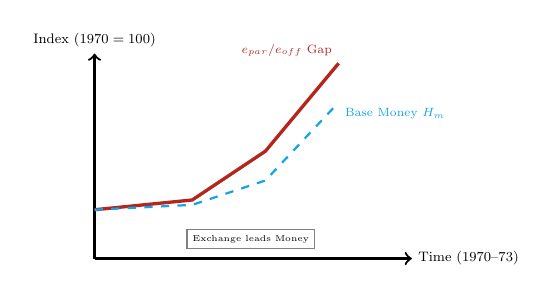
\begin{tikzpicture}[scale=0.62, every node/.style={transform shape}]
\draw[->, thick] (0,0) -- (6.5,0) node[right] {\footnotesize Time (1970--73)};
\draw[->, thick] (0,0) -- (0,4.2) node[above] {\footnotesize Index ($1970=100$)};
\draw[very thick, BrickRed] (0,1) -- (2,1.2) -- (3.5,2.2) -- (5,4.0) node[above left, font=\scriptsize] {$e_{\text{par}} / e_{\text{off}}$ Gap};
\draw[thick, Cerulean, dashed] (0,1) -- (2,1.1) -- (3.5,1.6) -- (5,3.2) node[below right, font=\scriptsize] {Base Money $H_m$};
\node[font=\tiny, fill=white, draw=gray] at (3.2,0.4) {Exchange leads Money};
\end{tikzpicture}
\caption{Fact 1: Exchange Rate leads Money}
\end{subfigure}
\hfill
\begin{subfigure}[b]{0.48\textwidth}
\centering
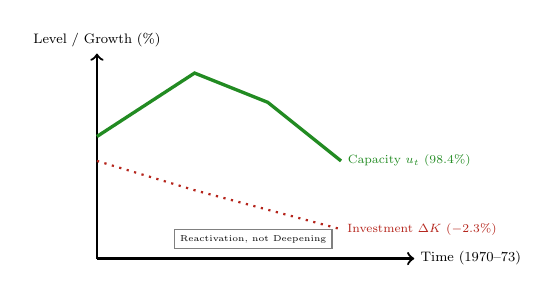
\begin{tikzpicture}[scale=0.62, every node/.style={transform shape}]
\draw[->, thick] (0,0) -- (6.5,0) node[right] {\footnotesize Time (1970--73)};
\draw[->, thick] (0,0) -- (0,4.2) node[above] {\footnotesize Level / Growth (\%)};
\draw[very thick, ForestGreen] (0,2.5) -- (2,3.8) -- (3.5,3.2) -- (5,2.0) node[right, font=\scriptsize] {Capacity $u_t$ ($98.4\%$)};
\draw[thick, BrickRed, dotted] (0,2.0) -- (2,1.4) -- (3.5,1.0) -- (5,0.6) node[right, font=\scriptsize] {Investment $\Delta K$ ($-2.3\%$)};
\node[font=\tiny, fill=white, draw=gray] at (3.2,0.4) {Reactivation, not Deepening};
\end{tikzpicture}
\caption{Fact 2: Capacity Peak vs. Negative GFCF}
\end{subfigure}
\vspace{0.3cm}
\begin{subfigure}[b]{0.48\textwidth}
\centering
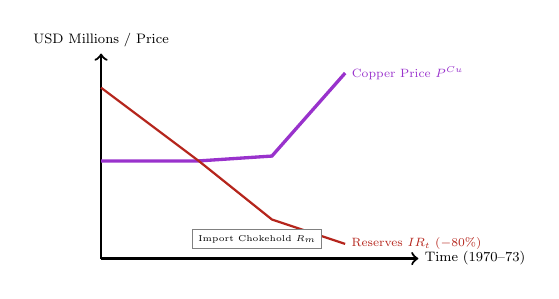
\begin{tikzpicture}[scale=0.62, every node/.style={transform shape}]
\draw[->, thick] (0,0) -- (6.5,0) node[right] {\footnotesize Time (1970--73)};
\draw[->, thick] (0,0) -- (0,4.2) node[above] {\footnotesize USD Millions / Price};
\draw[very thick, DarkOrchid] (0,2.0) -- (2,2.0) -- (3.5,2.1) -- (5,3.8) node[right, font=\scriptsize] {Copper Price $P^{\text{Cu}}$};
\draw[thick, BrickRed] (0,3.5) -- (2,2.0) -- (3.5,0.8) -- (5,0.3) node[right, font=\scriptsize] {Reserves $IR_t$ ($-80\%$)};
\node[font=\tiny, fill=white, draw=gray] at (3.2,0.4) {Import Chokehold $R_m$};
\end{tikzpicture}
\caption{Fact 3: Copper Boom vs. Reserve Drain}
\end{subfigure}
\hfill
\begin{subfigure}[b]{0.48\textwidth}
\centering
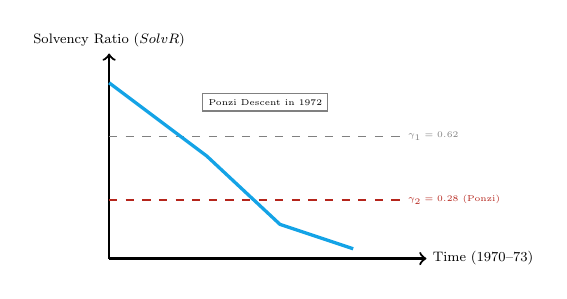
\begin{tikzpicture}[scale=0.62, every node/.style={transform shape}]
\draw[->, thick] (0,0) -- (6.5,0) node[right] {\footnotesize Time (1970--73)};
\draw[->, thick] (0,0) -- (0,4.2) node[above] {\footnotesize Solvency Ratio ($\text{SolvR}$)};
\draw[dashed, gray] (0,2.5) -- (6,2.5) node[right, font=\tiny] {$\gamma_1 = 0.62$};
\draw[dashed, BrickRed] (0,1.2) -- (6,1.2) node[right, font=\tiny] {$\gamma_2 = 0.28$ (Ponzi)};
\draw[very thick, Cerulean] (0,3.6) -- (2,2.1) -- (3.5,0.7) -- (5,0.2);
\node[font=\tiny, fill=white, draw=gray] at (3.2,3.2) {Ponzi Descent in 1972};
\end{tikzpicture}
\caption{Fact 4: Central Bank Solvency Trajectory}
\end{subfigure}
\caption{Visual-First Stylized Facts of the Unidad Popular Macroeconomic Trajectory (1970--1973).}
\label{fig:stylized_facts_2x2}
\end{figure}

\subsection{Neo-Lakatosian Tournament Design and Competing Causal Orderings}
\label{sec:tournament_design}

\textbf{4.6} Following \citet{KingSznajder2006}, we operationalize the three rival traditions as competing causal structures characterized by distinct zero restrictions on temporal precedence:

\begin{figure}[H]
\centering
\begin{subfigure}[b]{0.32\textwidth}
\centering
\begin{tikzpicture}[scale=0.75, every node/.style={transform shape, font=\footnotesize}]
\node[draw, rectangle, rounded corners, fill=panel, align=center] (def) at (0,3) {Fiscal\\Deficit};
\node[draw, rectangle, rounded corners, fill=panel, align=center] (gm) at (0,1.5) {Money\\Growth ($g_M$)};
\node[draw, rectangle, rounded corners, fill=panel, align=center] (pi) at (0,0) {Inflation\\($\pi$)};
\draw[-{Latex[length=2mm]}, thick] (def) -- (gm);
\draw[-{Latex[length=2mm]}, thick] (gm) -- (pi);
\end{tikzpicture}
\caption{$H_1$: Monetarist}
\end{subfigure}
\begin{subfigure}[b]{0.32\textwidth}
\centering
\begin{tikzpicture}[scale=0.75, every node/.style={transform shape, font=\footnotesize}]
\node[draw, rectangle, rounded corners, fill=panel, align=center] (cr) at (0,3) {Artificial\\Credit};
\node[draw, rectangle, rounded corners, fill=panel, align=center] (inv) at (0,1.5) {Malinvestment\\($\Delta K \gg 0$)};
\node[draw, rectangle, rounded corners, fill=panel, align=center] (bust) at (0,0) {Bust / Velocity\\Collapse ($v$)};
\draw[-{Latex[length=2mm]}, thick] (cr) -- (inv);
\draw[-{Latex[length=2mm]}, thick] (inv) -- (bust);
\end{tikzpicture}
\caption{$H_2$: Austrian ABCT}
\end{subfigure}
\begin{subfigure}[b]{0.34\textwidth}
\centering
\begin{tikzpicture}[scale=0.75, every node/.style={transform shape, font=\footnotesize}]
\node[draw, rectangle, rounded corners, fill=panelb, align=center] (ext) at (-1.2,3) {World Money\\Shocks ($g_e, g_{IR}$)};
\node[draw, rectangle, rounded corners, fill=panelb, align=center] (dist) at (1.2,3) {Distributive\\Conflict ($\omega$)};
\node[draw, rectangle, rounded corners, fill=panelc, align=center] (solv) at (-1.2,1.5) {Solvency\\$\text{SolvR}_t \le \gamma_S$};
\node[draw, rectangle, rounded corners, fill=panelc, align=center] (gm3) at (1.2,1.5) {LLR Money\\Accom. ($g_M$)};
\node[draw, rectangle, rounded corners, fill=stress, align=center] (pi3) at (0,0) {Regime Inflation\\$\pi_t(\text{SolvR})$};
\draw[-{Latex[length=2mm]}, thick] (ext) -- (solv);
\draw[-{Latex[length=2mm]}, thick] (dist) -- (gm3);
\draw[-{Latex[length=2mm]}, thick] (solv) -- (pi3);
\draw[-{Latex[length=2mm]}, thick] (gm3) -- (pi3);
\draw[-{Latex[length=2mm]}, dashed] (pi3) to [bend right=45] (gm3);
\end{tikzpicture}
\caption{$H_3$: Structural-Dependency}
\end{subfigure}
\caption{Causal Directed Acyclic Graphs (DAGs) of the Competing Research Traditions.}
\label{fig:causal_dags}
\end{figure}

\begin{table}[H]
\centering
\small
\caption{Hypothesis Tournament Zero Restrictions and Empirical Decision Rules}
\label{tab:tournament_restrictions}
\begin{tabular}{p{3.2cm}p{3.8cm}p{3.8cm}p{3.8cm}}
\toprule
\textbf{Dimension} & \textbf{$H_1$: Monetarist \citep{Edwards2024}} & \textbf{$H_2$: Austrian \citep{EspinosaVejar2025}} & \textbf{$H_3$: Structural-Dependency (Ours)} \\
\midrule
\textbf{Hard Core} & Exogenous money printing; quantity theory pass-through. & Artificial credit causes malinvestment; inevitable bust. & Endogenous money accommodation under world-money constraint. \\
\textbf{Accommodation Restriction} & $H_0: \pi_{t-1} \to g_M = 0$ (Money is not accommodated). & $H_0: \pi_{t-1} \to g_M = 0$ (Credit is uncaused driver). & \textbf{Reject $H_0$}: $\pi_{t-1} \to g_M > 0$ ($p < 0.001$, central bank accommodates). \\
\textbf{Transmission Speed} & Fast 1-year pass-through: $g_{M,t-1} \to \pi_t > 0$. & Fast credit transmission into prices and capital. & \textbf{Delayed}: $g_{M,t-1}$ inert; transmission delayed to lag 2 ($p = 0.008$). \\
\textbf{Capital Deepening} & Output boom is short-run monetary illusion. & \textbf{Requires}: Gross fixed investment spikes ($\Delta K \gg 0$). & \textbf{Idle capacity}: $\Delta K \le 0$ while capacity utilization $u \uparrow 98.44\%$. \\
\textbf{Threshold Non-Linearity} & Linear pass-through across all reserve levels ($\beta_1 = \beta_2$). & Linear price distortion driven by credit and velocity. & \textbf{Regime shift}: $\beta_{\text{Ponzi}} \gg \beta_{\text{Hedge}} \approx 0$ at $\text{SolvR}_t \le \gamma_S$. \\
\bottomrule
\end{tabular}
\end{table}

\subsection{Econometric Methodology: The Monthly Threshold VAR Specification}
\label{sec:tvar_methodology}

\textbf{4.7} To evaluate the non-linear regime-switching dynamics of $H_3$, we implement a Threshold Vector Autoregressive model (TVAR) following the econometric framework of \citet{ClavijoCortesKappesRochon2025}. High-frequency monthly data ($N \approx 240$, 1960--1980) provides the degrees of freedom required to estimate multi-regime models without cell-size collapse under standard sample trimming ($\epsilon = 0.15$).

\textbf{4.8} The monthly TVAR system is specified as:
\begin{equation}
y_m = \sum_{k=1}^K \left[\Pi_{c,k} + \sum_{j=1}^p \Pi_{j,k} y_{m-j} + e_{m,k}\right] I\{\gamma_{k-1} < \text{SolvR}_{m-d} \le \gamma_k\}
\label{eq:tvar_model}
\end{equation}
where:
\begin{itemize}[leftmargin=2em]
	\item $y_m = [\text{CapImp}_m,\; \text{FiscalDeficit}_m,\; g_{H,m},\; \pi_m]'$ is the endogenous vector containing import capacity growth, fiscal deficit share, base money growth, and CPI inflation.
	\item $\text{SolvR}_{m-d} \equiv \frac{e_{m-d} \cdot IR_{m-d}}{M_{m-d}}$ is the lagged threshold variable governing regime transitions.
	\item $K \in \{1, 2, 3\}$ allows nested testing of a \textbf{3-Regime TVAR} (Hedge vs. Speculative vs. Ponzi) against a \textbf{2-Regime TVAR} (Solvent vs. Insolvent) and the \textbf{1-Regime Linear Null}.
	\item $\Pi_{c,k}$ and $\Pi_{j,k}$ are regime-specific constant vectors and lag coefficient matrices.
	\item $e_{m,k} \sim \mathcal{N}(0, \Sigma_k)$ captures heteroscedastic covariance structures across regimes.
\end{itemize}

\textbf{4.9} Identification of structural shocks is achieved through a recursive Cholesky decomposition ordering:
\begin{equation}
\text{Import Capacity } (\text{CapImp}_m) \longrightarrow \text{Fiscal Deficit } (\text{Def}_m) \longrightarrow \text{Base Money } (g_{H,m}) \longrightarrow \text{CPI Inflation } (\pi_m)
\end{equation}
This ordering reflects the structural political economy sequence: external import bottlenecks and fiscal constraints are determined first, the central bank adjusts liquidity ($g_H$) as an intermediate accommodation instrument, and prices ($\pi$) register the final systemic response.

\textbf{4.10} Following \citet{Koop1996} and \citet{ClavijoCortesKappesRochon2025}, we compute regime-dependent Generalized Impulse Response Functions (GIRFs) to trace how a monetary or external shock transmits conditionally when the economy resides in Hedge, Speculative, or Ponzi states.


\textbf{4.11} All nominal series pre-1975 are normalized across currency re-denominations ($1,000\text{ Old Pesos} \to 1\text{ Escudo}$ in 1960; $1,000\text{ Escudos} \to 1\text{ Modern Peso}$ in 1975). This multi-frequency dataset provides the empirical foundation for testing the tournament hypotheses.
